\section{Factory\-Base Class Reference}
\label{classFactoryBase}\index{FactoryBase@{FactoryBase}}
Inheritance diagram for Factory\-Base::\begin{figure}[H]
\begin{center}
\leavevmode
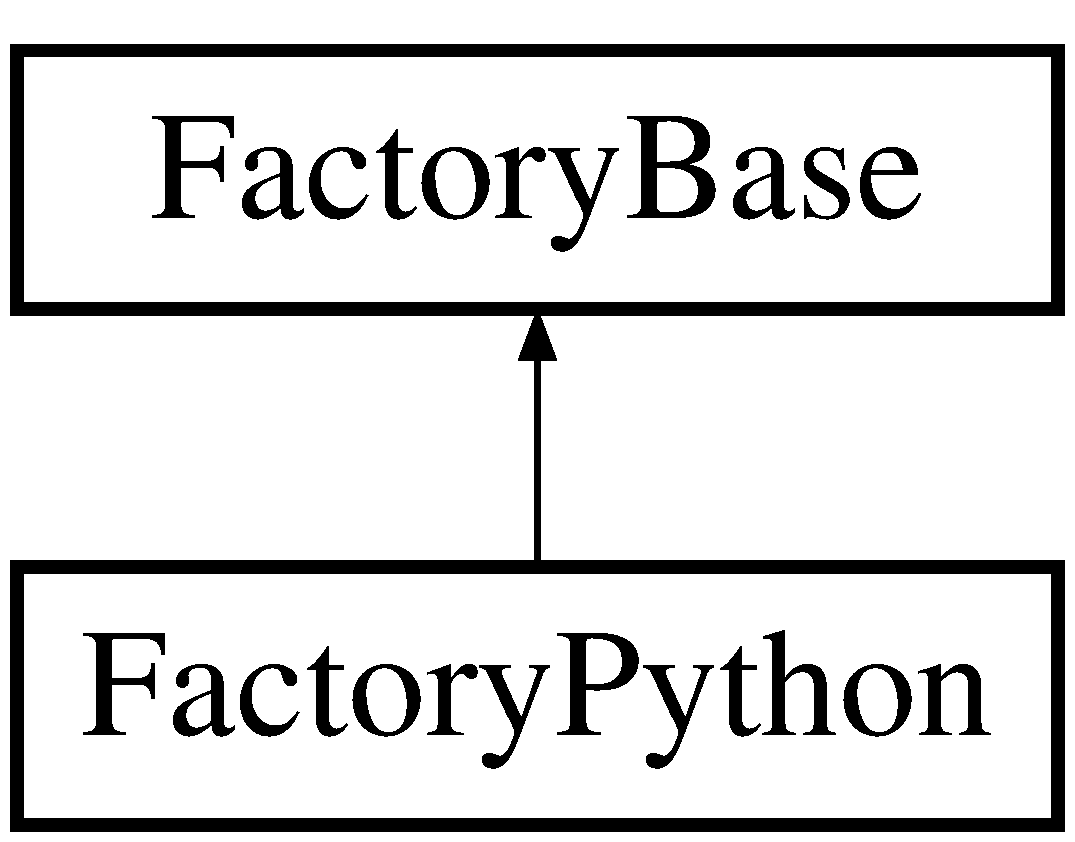
\includegraphics[height=2cm]{classFactoryBase}
\end{center}
\end{figure}
\subsection*{Public Member Functions}
\begin{CompactItemize}
\item 
{\bf \_\-\_\-init\_\-\_\-} (profile)
\begin{CompactList}\small\item\em Factory\-Base class constructor. \item\end{CompactList}\item 
{\bf \_\-\_\-dele\_\-\_\-} ()
\item 
{\bf create} (mgr)
\begin{CompactList}\small\item\em Create component. \item\end{CompactList}\item 
{\bf destroy} (comp)
\begin{CompactList}\small\item\em Destroy component. \item\end{CompactList}\item 
{\bf profile} ()
\begin{CompactList}\small\item\em Get component profile. \item\end{CompactList}\item 
{\bf number} ()
\begin{CompactList}\small\item\em Get number of component instances. \item\end{CompactList}\end{CompactItemize}


\subsection{Member Function Documentation}
\index{FactoryBase@{Factory\-Base}!__dele__@{\_\-\_\-dele\_\-\_\-}}
\index{__dele__@{\_\-\_\-dele\_\-\_\-}!FactoryBase@{Factory\-Base}}
\subsubsection{\setlength{\rightskip}{0pt plus 5cm}Factory\-Base::\_\-\_\-dele\_\-\_\- ()}\label{classFactoryBase_FactoryPythona4}


\index{FactoryBase@{Factory\-Base}!__init__@{\_\-\_\-init\_\-\_\-}}
\index{__init__@{\_\-\_\-init\_\-\_\-}!FactoryBase@{Factory\-Base}}
\subsubsection{\setlength{\rightskip}{0pt plus 5cm}Factory\-Base::\_\-\_\-init\_\-\_\- (profile)}\label{classFactoryBase_FactoryPythona3}


Factory\-Base class constructor. 

Factory\-Base class constructor. \begin{Desc}
\item[Parameters:]
\begin{description}
\item[{\em profile}]component profile\end{description}
\end{Desc}
\index{FactoryBase@{Factory\-Base}!create@{create}}
\index{create@{create}!FactoryBase@{Factory\-Base}}
\subsubsection{\setlength{\rightskip}{0pt plus 5cm}Factory\-Base::create (mgr)}\label{classFactoryBase_FactoryBasea2}


Create component. 

Create component implemented in Python. Pure virtual method. \begin{Desc}
\item[Parameters:]
\begin{description}
\item[{\em mgr}]{\bf Manager}{\rm (p.\,\pageref{classManager})} object\end{description}
\end{Desc}


Reimplemented in {\bf Factory\-Python} {\rm (p.\,\pageref{classFactoryPython_FactoryPythona1})}.\index{FactoryBase@{Factory\-Base}!destroy@{destroy}}
\index{destroy@{destroy}!FactoryBase@{Factory\-Base}}
\subsubsection{\setlength{\rightskip}{0pt plus 5cm}Factory\-Base::destroy (comp)}\label{classFactoryBase_FactoryBasea3}


Destroy component. 

Destroy component instance) Pure virtual method. \begin{Desc}
\item[Parameters:]
\begin{description}
\item[{\em comp}]Rtc\-Base object\end{description}
\end{Desc}


Reimplemented in {\bf Factory\-Python} {\rm (p.\,\pageref{classFactoryPython_FactoryPythona2})}.\index{FactoryBase@{Factory\-Base}!number@{number}}
\index{number@{number}!FactoryBase@{Factory\-Base}}
\subsubsection{\setlength{\rightskip}{0pt plus 5cm}Factory\-Base::number ()}\label{classFactoryBase_FactoryPythona6}


Get number of component instances. 

Get number of current component instances.\index{FactoryBase@{Factory\-Base}!profile@{profile}}
\index{profile@{profile}!FactoryBase@{Factory\-Base}}
\subsubsection{\setlength{\rightskip}{0pt plus 5cm}self \_\-Profile Component Factory\-Base::profile ()}\label{classFactoryBase_FactoryPythona5}


Get component profile. 

Get component profile.

The documentation for this class was generated from the following file:\begin{CompactItemize}
\item 
{\bf Factory.py}\end{CompactItemize}
